%!TEX root = ./seminarpaper.tex

\chapter{Implemented Functions}

	This chapter gives an overview about all implemented functions. Figure \ref{fig:OverviewProbabilityDistributions} on page \pageref{fig:OverviewProbabilityDistributions} shows all of them.

	\begin{figure}[h]
		\centering
		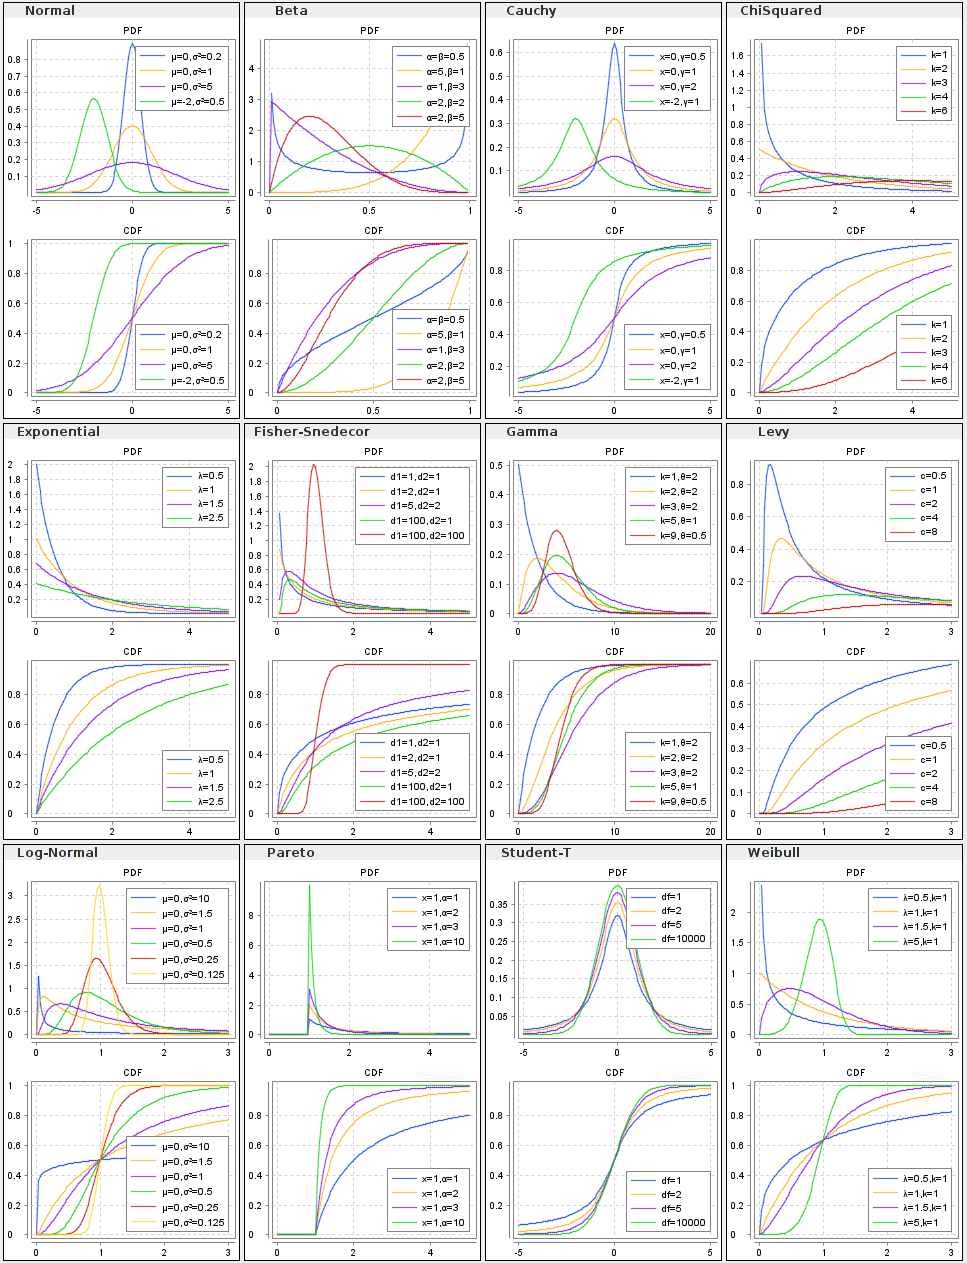
\includegraphics[width=1\textwidth]{Figures/OverviewProbabilityDistributions}~\\
		\caption{Overview Probability Distributions}
		\url{https://commons.apache.org/proper/commons-math/userguide/distribution.html}
		\label{fig:OverviewProbabilityDistributions}
	\end{figure}

	\section{Beta}

		The beta distribution has two parameters $\alpha > 0$ and $\beta > 0$ and is defined on the interval $[0,1]$. The \ac{PDF} of the beta distribution is defined as
		\\
		$$f(x) = \frac{x^{\alpha-1}(1-x)^{\beta-1}}{B(\alpha,\beta)}  \hspace{.3in} 0 \le x \le 1; \alpha, \beta > 0$$
		\\
		with the beta function $B$ as a normalization constant to ensure that the total probability integrates to 1. The formula of the beta function is defined as
		\\
		$$B(\alpha,\beta) = \frac{\Gamma(\alpha)\Gamma(\beta)}{\Gamma(\alpha + \beta)}$$
		\\
		where $\Gamma$ is the gamma function. The \ac{CDF} of the beta distribution is defined as
		\\
		$$F(x) = I_{x}(\alpha,\beta) = \frac{\int_{0}^{x}{t^{\alpha-1}(1-t)^{\beta-1}dt}}{B(\alpha,\beta)} \hspace{.2in} 0 \le x \le 1; \alpha, \beta > 0$$

	\section{Cauchy}

	\section{ChiSquared}

	\section{Exponential}

	\section{Fisher-Snedecor}

	\section{Gamma}

	\section{Levy}

	\section{Log-Normal}

	\section{Normal}

	\section{Pareto}

	\section{Student-T}

	\section{Weibull}